\section{Evidence Dependencies, Threat Propagation, and Dynamic Reasoning}

\subsection{A Typed Object-Dependency Graph}

OAL classifies claims; a dependency graph records relations relevant to their appraisal. Let $G_t=(V_t,E_t)$ be a time-indexed directed multigraph whose vertices denote the four object types, with version or state-interval identifiers where applicable. Relations have declared source and target types: an entity \textit{controls} a platform; a platform \textit{hosts} another device or a model artifact; a platform \textit{produces} an observation product; a path \textit{transmits} a product; an entity \textit{endorses} or \textit{consumes} a product; and a ledger-record product \textit{commits to} another product. A derived product \textit{depends on} input products through an identified transformation. Each transformation identifier links all inputs, outputs, the executing platform, responsible entity, code/model version, and event-time interval. A W3C PROV serialization can represent that transformation as an activity node \citep{w3c2013provdm}; activities describe relations among the four OAL object types. An OAL entity corresponds to a responsible principal, usually a PROV agent, while a data product corresponds to a PROV entity. Time and version qualifiers are essential. A decision based on model version 4.2 before a rollback requires that version and activity interval to qualify the relation ``UAV-7 hosts model M.''

\begin{figure}[!htbp]
\centering
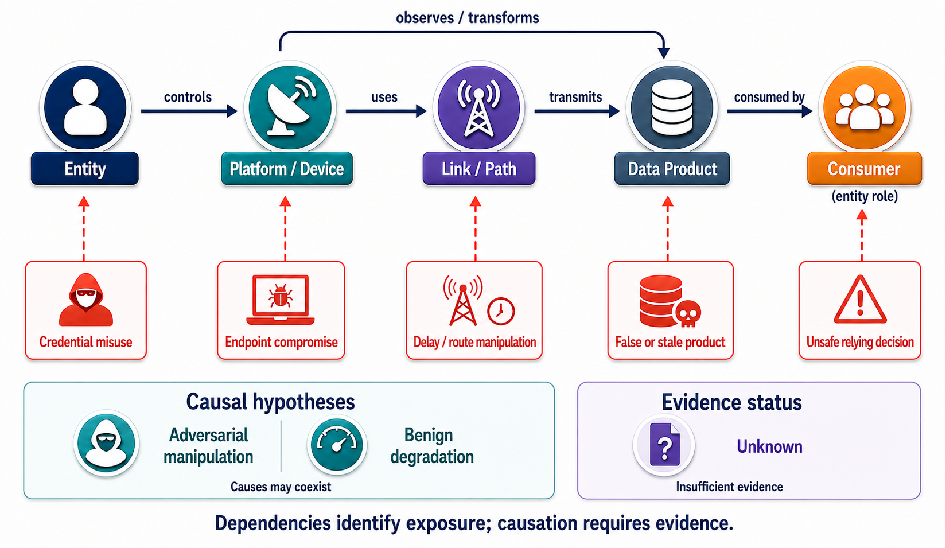
\includegraphics[width=\textwidth]{figures/figure-04-dependency-threat.pdf}
\caption{Simplified object dependencies and illustrative exposures. Solid arrows name operational relations; red dashed arrows associate an exposure with its object. The lower panels distinguish causal hypotheses from the epistemic status of the evidence. Causal propagation claims require explicit causal evidence and inference rules.\label{fig:dependency}}
\end{figure}

The graph supports evidence tracing and exposure analysis. A fresh attestation can support a scoped claim about measured platform state; verified provenance supports recorded derivation; corroborating observations support physical plausibility under their dependence assumptions. Each inference requires an explicit rule connecting evidence to a property. Hosting and transmission relations identify operational dependencies; inference about a property or causal effect requires a specified model. Compromised credentials may permit device access; a compromised device may alter observations; a manipulated path may delay delivery or substitute content if authentication fails; and a consumer may then act on the result. Figure~\ref{fig:dependency} depicts this conditional chain. Traversal follows declared relation semantics to identify claims for reassessment; score updates depend on the specified inference model. If a causal or probabilistic model is used, its conditional structure, common causes, and parameters must be specified separately. Versioning and event ordering expose feedback cycles so that update rules can preserve the identity and dependence of recirculated evidence.

\subsection{A Unified Threat-Analysis Sentence}

Every scenario should be expressible as: \emph{an attacker with capability $C$ acts on object $O$, propagates through relations $P$, creates mission impact $I$, and is constrained or detected by controls $K$ under assumptions $A$}. This grammar connects threat catalogs to assurance cases and exposes missing controls. Table~\ref{tab:threats} applies the grammar to common public scenarios at a capability level suitable for reproducible defensive analysis.

\begin{table}[!htbp]
\caption{Object-centered threat, degradation, and evidence-absence analysis.\label{tab:threats}}
\begin{adjustwidth}{-\extralength}{0cm}
\scriptsize
\begin{tabularx}{\fulllength}{@{}P{24mm}P{29mm}P{34mm}YY@{}}
\toprule
\textbf{Class and initial object} & \textbf{Capability or condition} & \textbf{Propagation path} & \textbf{Mission impact} & \textbf{Controls and residual uncertainty}\\
\midrule
Malicious/entity & Stolen or misused credential & controls device $\rightarrow$ endorses product $\rightarrow$ record accepted & Unauthorized tasking or false accountability & Short-lived delegation, multi-party approval, behavioral evidence, rapid revocation; valid credentials can still mask insider intent\\
Malicious/device & Capture, malware, or model replacement & hosts sensor/model $\rightarrow$ observes/transforms data & Consistent but false products across many consumers & Attestation, key protection, diversity, provenance, quarantine; measured components may omit sensors or runtime behavior\\
Malicious/link & Jamming, wormhole, selective forwarding, replay & transmits/custodies data $\rightarrow$ delays or substitutes version & Loss of availability, stale situational picture, biased fusion & Link context, authenticated sequence, path diversity, freshness policy; attribution remains uncertain\\
Malicious/data & False-data injection, poisoning, semantic manipulation & transformed / endorsed / recorded product $\rightarrow$ consumed decision & Incorrect classification, route, or resource allocation & Physical plausibility, independent modality, robust fusion, lineage; independence assumptions can fail\\
Benign environment & Fading, multipath, weather, occlusion, low energy & environmental conditions degrade link or observation evidence & Delay, disagreement, reduced coverage & Environment-aware baselines, graceful degradation, explicit ``benign-degraded'' hypothesis; models may be incomplete\\
Evidence absence & Disconnection, failed verifier, missing lineage, stale clock & prevents appraisal across several relations & Unsafe overconfidence or unnecessary isolation & Unknown state, bounded authority, conservative policy, later reconciliation; compromise attribution requires additional evidence\\
\bottomrule
\end{tabularx}
\end{adjustwidth}
\end{table}

Three labels organize the interpretation of an anomaly. \emph{Malicious} denotes evidence supporting intentional or adversarial manipulation; \emph{benign-degraded} denotes a supported environmental or operational explanation; and \emph{unknown} denotes insufficient evidence to resolve the explanation. Unknown describes the evidence status of an assessment. Operational states additionally include nominal operation and recovery, and malicious action can coincide with environmental degradation. For example, packet loss may justify restricting reliance on a path, while attribution of attacker intent requires separate support. Recovery tracks review of cached data, keys, neighbors, and prior decisions after software is re-attested. Policies map the assessed properties, uncertainty, and recovery status to bounded actions---continue, reduce privilege, request corroboration, isolate, return, or escalate to a human.

\subsection{The CTG Reasoning Loop}

CTG-Trust is the context--temporal--graph workflow developed in this synthesis and shown in Figure~\ref{fig:ctg}. The workflow specifies inputs and decision records for implementations with selected and validated inference and policy mechanisms. First, evidence events are captured with source, subject, event and receipt times, clock uncertainty, context, value, and lineage. Second, evidence reliability and dependencies are appraised: a device self-report and an external verifier carry different evidential relationships. Third, a selected method assesses a named object property. Fourth, graph traversal identifies downstream claims requiring reassessment and shared causes beyond the local assessment. Fifth, the assessment is revised as needed and its uncertainty made explicit. Sixth, a mission policy chooses an action. Seventh, the decision, relevant versions, and evidence commitment are recorded for review. Eighth, independently appraised outcomes and later verification update the evidence base, with ground-truth labels established independently of the workflow's decisions.

\begin{figure}[!htbp]
\centering
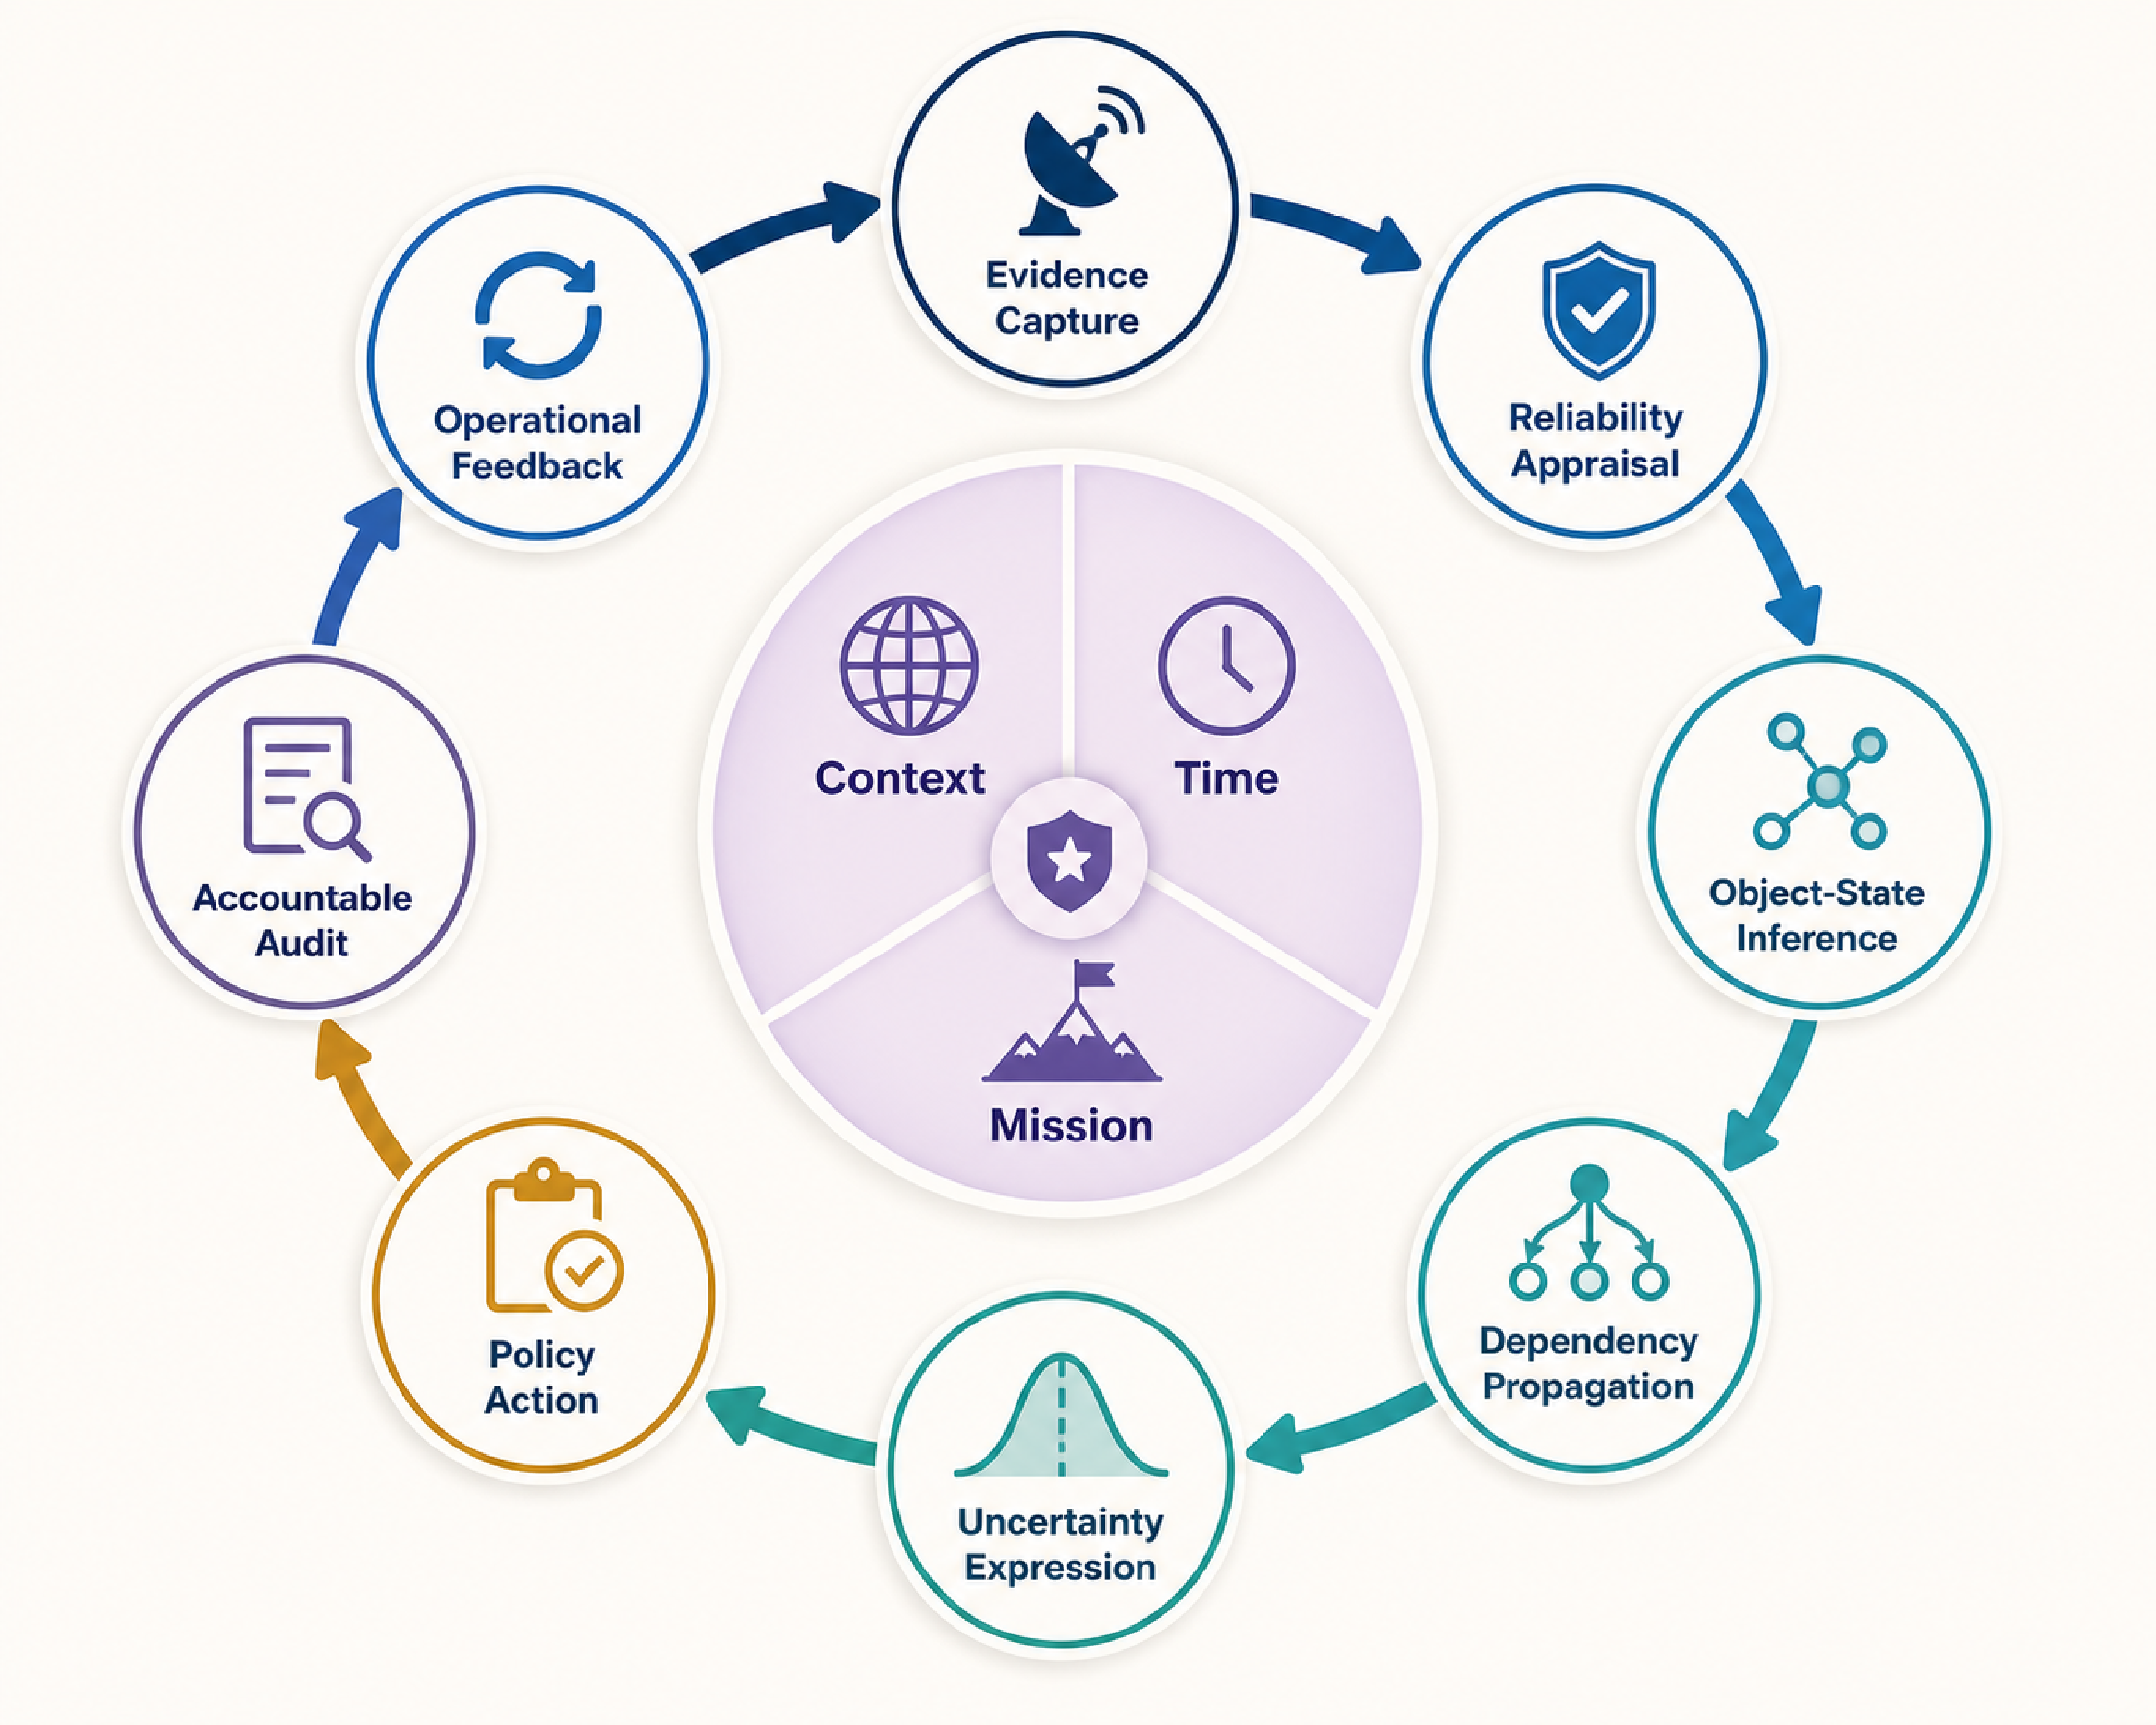
\includegraphics[width=0.86\textwidth]{figures/figure-05-ctg-reasoning-loop.pdf}
\caption{CTG workflow for evidence appraisal, dependency review, uncertainty representation, policy action, and audit. The diagram specifies information flow; performance depends on the selected methods and their mission-specific validation.\label{fig:ctg}}
\end{figure}

Evidence reuse requires special care. A gateway's report can influence device reputation, link assessment, data quality, and a fused decision; treating the resulting scores as independent can count the same observation repeatedly. Implementations retain unique evidence identifiers, parent identifiers, and shared calibration, localization, model, operator, and relay dependencies. Exact duplicates contribute once to a given update. Distinct observations with shared causes require a joint model or a method with stated dependence assumptions; any discounting rule requires justification under those assumptions. For unresolved dependence, a policy may classify the evidence as potentially dependent or request another source. Statistical independence requires assessment of shared navigation references, training data, and environments, including across distinct identities or organizations. Ledger persistence preserves the recorded lineage for appraisal, subject to capture completeness.

\subsection{A Bounded Decision Trace}

A constructed policy example illustrates how a USV gateway assesses a target-location product for UUV route replanning. Its thresholds specify the example; operational use requires mission-specific selection and validation. Policy version $p_7$ requires an unexpired delegation, verified product provenance, an accepted platform appraisal, acquisition age at most $60$ s including clock uncertainty, and corroboration independent of the identified common localization failure. Replanning requires every gate to pass, with freshness and observation validity assessed alongside the ledger commitment.

At decision time, the gateway has a signed observation $d_1$ with an acquisition-age interval of $[42,48]$ s, a fused product $d_2$ whose only observation parent is $d_1$, and an observation $d_3$ from a second vehicle with age interval $[58,66]$ s. The authorization, provenance, and platform-appraisal gates are assumed to pass. The lineage shows that $d_1$ and $d_2$ supply one observation lineage, while $d_3$ uses the same localization reference as $d_1$. The decision trace is then reproducible: $d_1$ passes freshness; $d_2$ reuses the same observation lineage; and $d_3$ exceeds the worst-case freshness bound while retaining the shared localization concern. The gateway records the target-location claim as requiring further support and selects the preauthorized local fallback specified by $p_7$ in place of replanning. The decision rests on evidence sufficiency; attribution of malicious behavior is a separate assessment.

The audit record contains the gate results, lineage identifiers, assessed uncertainty, policy and platform-appraisal versions, delegated-authority basis, and selected fallback. A fresh observation with an adequately justified independent localization basis would trigger reassessment. Observation age and independence retain their acquisition and lineage meanings when ledger inclusion occurs later. This trace makes the framework operational at the level of a reviewable decision procedure while leaving threshold selection, fallback safety, and mission-loss evaluation to an implementation study.

\subsection{Trust Methods and Appropriate Claims}

The literature offers several method families, summarized in Table~\ref{tab:trust-methods}. Each expresses a different claim under different assumptions. The qualitative comparison provides a selection guide for future mission-specific validation.

\begin{table}[!htbp]
\caption{Trust-inference families and their role in CTG.\label{tab:trust-methods}}
\begin{adjustwidth}{-\extralength}{0cm}
\small
\begin{tabularx}{\fulllength}{@{}P{30mm}P{40mm}YYY@{}}
\toprule
\textbf{Family} & \textbf{Useful representation} & \textbf{Strength} & \textbf{Critical assumption/risk} & \textbf{Representative sources}\\
\midrule
Weighted multi-attribute score & Context-weighted evidence features & Interpretable and implementable at constrained edges & Weights and thresholds can be arbitrary or task-insensitive & \citep{ahmed2019trust,aaqib2023iot}\\
Probabilistic trust/reputation & Evidence-updated belief or behavior propensity & Supports sequential assessment when the update model is specified & Priors, dependence, and behavior persistence require justification & \citep{mui2003computational}\\
Subjective logic & Belief, disbelief, uncertainty, and base rate & Makes ignorance visible and supports opinion combination & Dependence and source identity must be handled explicitly & \citep{jsang2016subjective}\\
State-space/Markov & Latent state with temporal transitions & Represents persistence and recovery & State meanings and transition parameters need mission data & \citep{arifeen2020hidden}\\
Rule/tree/fuzzy methods & Human-readable rules or learned partitions & Can combine heterogeneous evidence & Coverage gaps and abrupt boundaries; calibration often unclear & \citep{jiang2020dynamic,zhu2024design}\\
Machine/deep learning & Learned anomaly or multi-view representation & Captures nonlinear patterns & Shift, poisoning, explainability, and overconfidence & \citep{shafique2021detecting,dang2022deep,liu2022trusted}\\
Graph-based propagation & Relational evidence over dependencies & Connects local evidence to downstream exposure & Correlation, cycles, and collusion can amplify error & \citep{kamvar2003eigentrust,bellini2020blockchain}\\
\bottomrule
\end{tabularx}
\end{adjustwidth}
\end{table}

The underwater studies provide concrete examples of these model assumptions and their evaluation conditions. The HMM proposal in \citet{arifeen2020hidden} maps packet-loss rate and packet-error rate to latent malicious/trustworthy states; its MATLAB illustration uses ten observations with randomly initialized probabilities and demonstrates a temporal construction under a synthetic numerical setup. TEUC combines data-, link-, and node-based evidence with a C4.5 tree and reward/penalty updates \citep{jiang2020dynamic}. The study identifies acoustic loss as a reason normal nodes may receive low trust and assumes attack-free initial deployment so that the initial training evidence is unpolluted; its MATLAB simulation is conditioned on that setup. The broader UWSN review identifies evidence collection, evaluation, propagation, and updating as distinct design choices \citep{zhu2024design}. Together, these studies motivate three CTG requirements: keep node behavior distinct from sensor truth, assess attack classification alongside mission decision loss, and retain benign degradation as a possible explanation.

Equation~\eqref{eq:trust} provides an assessment interface for these methods when the output states the assessed property, context, horizon, uncertainty representation, and supporting validation. Probabilities require an event definition and calibration assessment; ordinal scores require an ordering interpretation and justified thresholds. Spectral reputation, such as EigenTrust, expresses relative reputation; its use as a mission-success probability would require an explicit event model and calibration \citep{kamvar2003eigentrust}. The reliance policy separately specifies authority, constraints, and decision consequences. Beta parameters, hidden-state transitions, scoring thresholds, message schemas, and performance targets remain empirical design choices for each implementation study.
